\section{Results}

To evaluate the performance of both models, several inferencing tests were conducted to see if the models had learned the latent features correctly.

\subsection{Recreation from the Training Dataset}

From each training dataset, a random frame was selected and passed through each model, loudness and F0 were kept constant. The results of the inferencing were then compared to the original training dataset.

Each model was able to successfully recrete original frames, though the Taylor Swift dataset yielded the best results.

Timbral features were slightly distorted (moreso with the Coldplay dataset) but the overall quality was good and it was easy to tell it was the original singer in both cases. Pitch estimation was highly accurate and in-line with the original pitch. This can be partially attributed to the accruacy of the CREPE pitch detection model\cite{CREPE} and because pitch was directly passed to the harmonic synthesiser.

A far bigger achievement was the re-synthesis of understandable words from the original frame. The original singing DDSP paper\cite{SingingDDSP} suffered a problem of stuttering when attempting resynthesis as their model was unable to recreate phonemes of the human voice accurately. It is possible that using a far larger datasets has improved the quality of the resynthesis because the models had become more general in their ability to synthesize the human voice. It must be said though that the Coldplay model was harder to understand.

\begin{figure}[H]
    \centering
    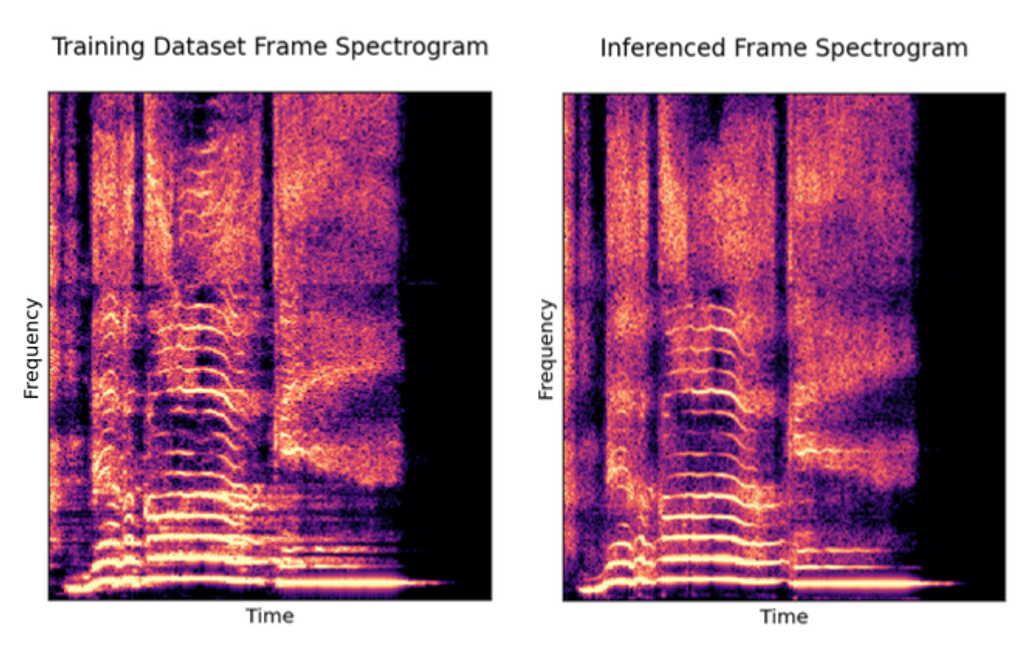
\includegraphics[width=0.8\textwidth]{research/results/TaylorSwift/InferredRecreation.png}
    \caption{(Taylor Swift) Original and resynthesized frames without latent modification}
\end{figure}

\begin{figure}[H]
    \centering
    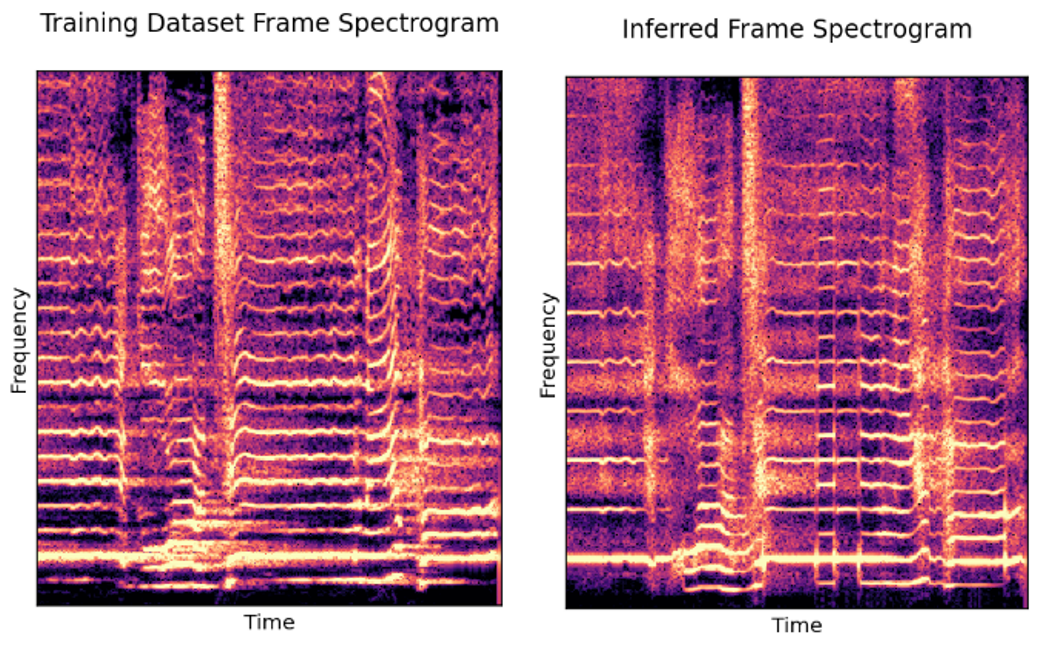
\includegraphics[width=0.8\textwidth]{research/results/Coldplay/InferredRecreation.png}
    \caption{(Coldplay) Original and resynthesized frames without latent modification}
\end{figure}

\subsection{F0 Pitch Transposition by a fixed octave}

A more advanced inferencing test was then undertaken, the fundamental frequency latent as determined by CREPE was transposed by fixed octaves (-2, -1, 0, 0.5, 1, 2) and the inferencing was re-preformed on the transposed latents. Both models responded to the change in F0 and were able to accurately transpose harmonic pitch by the correct octave amount. At minor transpositions, eg +1 or -1 octave, the resynthesized frame still sounded rather like a human voice. At greater transpositions it sounded like the noise and harmonic components were separate sources and did not constitute one voice.

As expected, modifying F0 did not change the pitch of the filtered noise at all, confirming that the pitch change had been directly passed to the harmonic synthesiser. This is interesting because we would have expected a little bit of distortion in the original pitch.

At extreme transpositions, harmonics sometimes appeared to go silent. The resynthesis then appeared to sound like a whisper, coming almost entirely out of the filtered noise. whispering occurs when the vocal chords are hold rigid preventing them from vibrating and producing sinusoidal sounds (harmonics in the case of singing). The fact the the models's output sounded like a whisper is a good sign that the model was able to learn and destinguish the noise and harmonics as per the Harmonic Plus Noise Model\cite{HarmonicPlusNoise}\cite{OriginalDDSP}.

\begin{figure}[H]
    \centering
    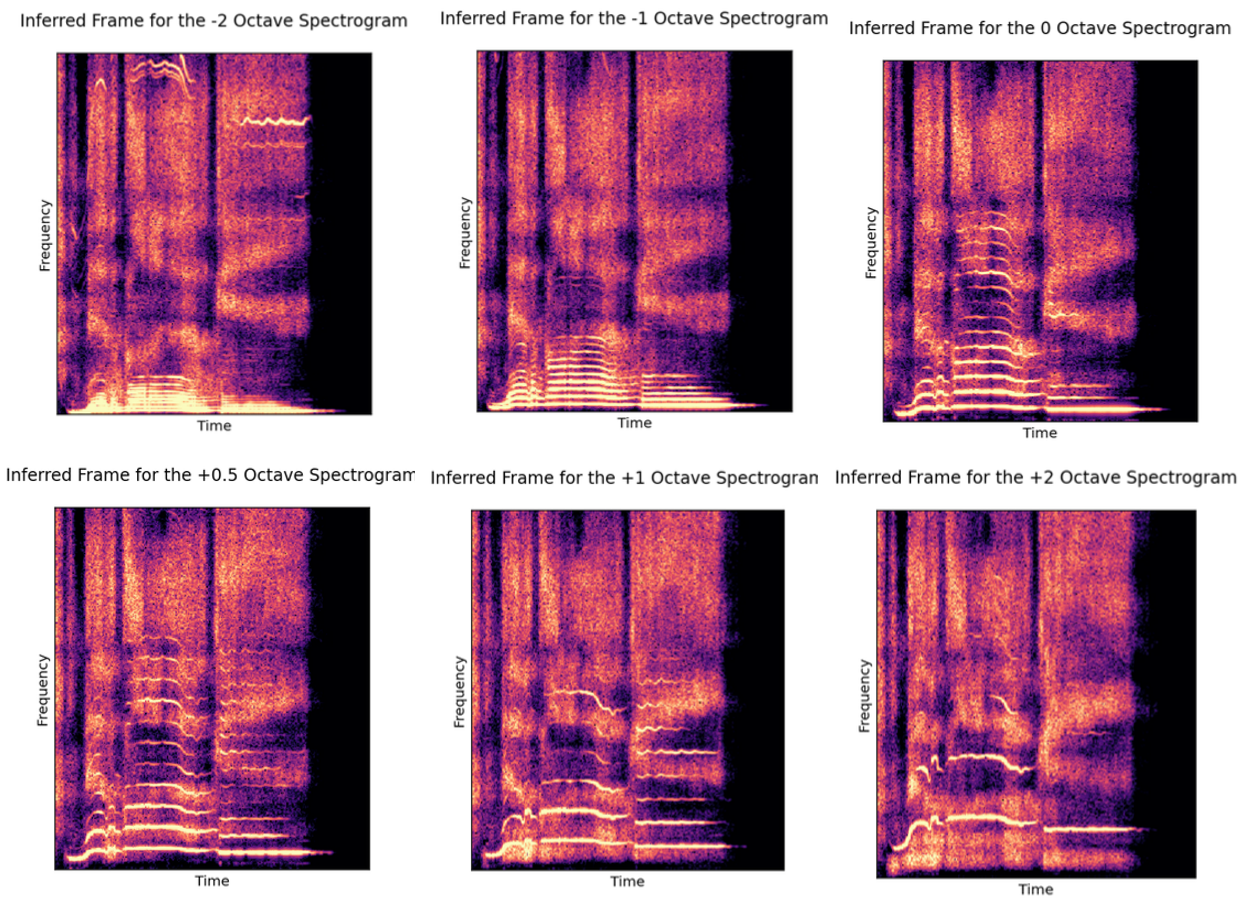
\includegraphics[width=\textwidth]{research/results/TaylorSwift/InferredTranspositions.png}
    \caption{(Taylor Swift) Inferred spectrogram frames at various octave transpositions realative to F0 at a certain timegrame in the original frame}
\end{figure}

\begin{figure}[H]
    \centering
    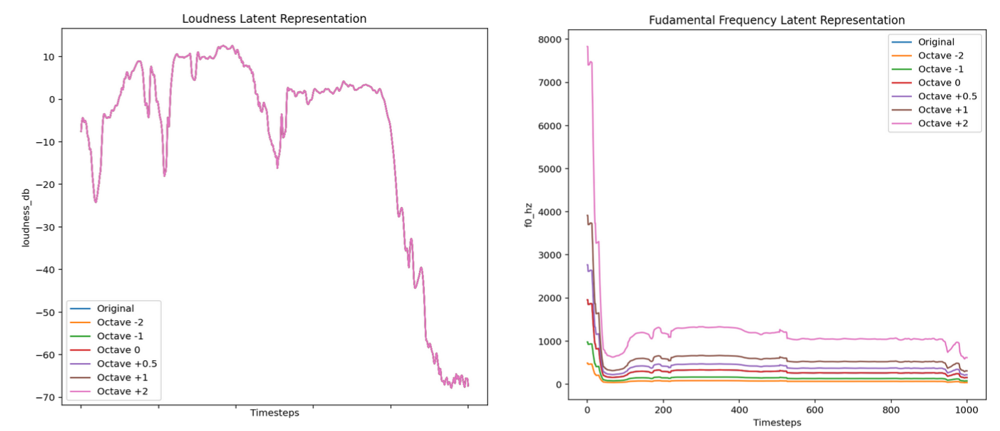
\includegraphics[width=\textwidth]{research/results/TaylorSwift/InferredTranspositionsGraphs.png}
    \caption{(Taylor Swift) Latent F0 and loudness features for various octave transpositions realative to F0 over timesteps throughout the frame}
\end{figure}

\begin{figure}[H]
    \centering
    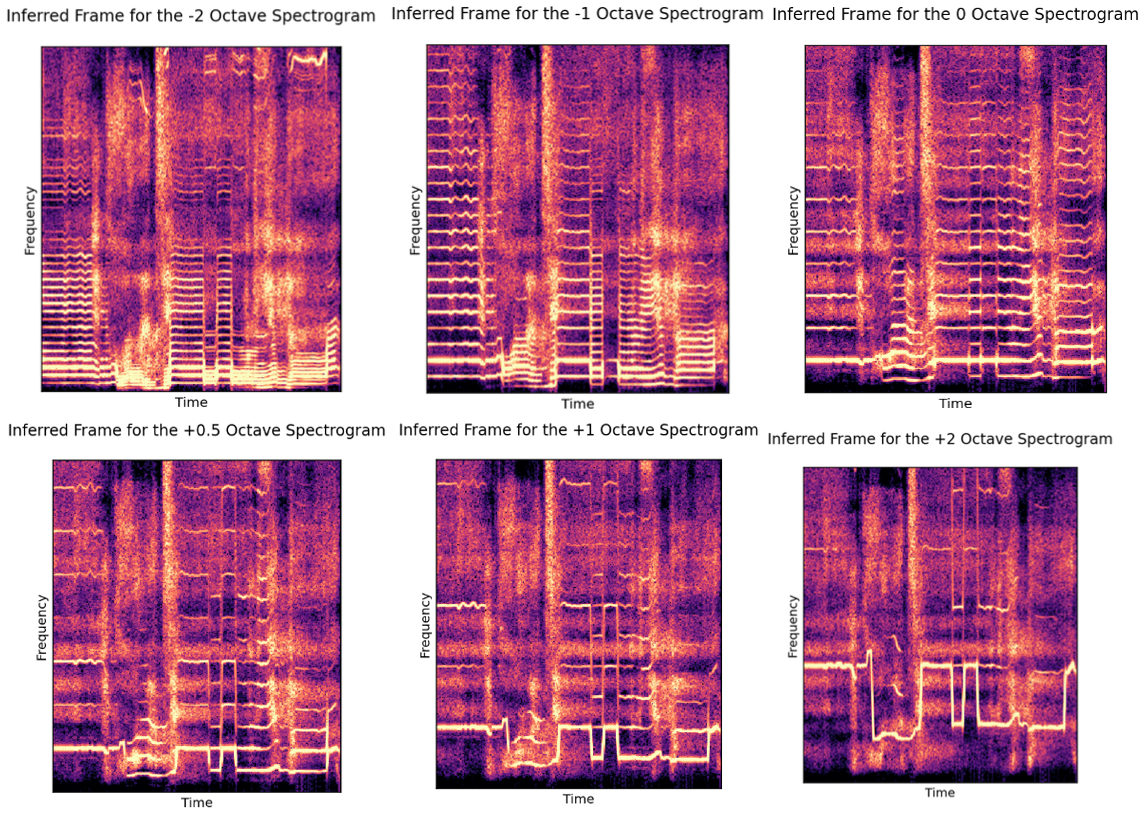
\includegraphics[width=\textwidth]{research/results/Coldplay/InferredTranspositions.png}
    \caption{(Coldplay) Inferred spectrogram frames at various octave transpositions realative to F0 at a certain timegrame in the original frame}
\end{figure}

\begin{figure}[H]
    \centering
    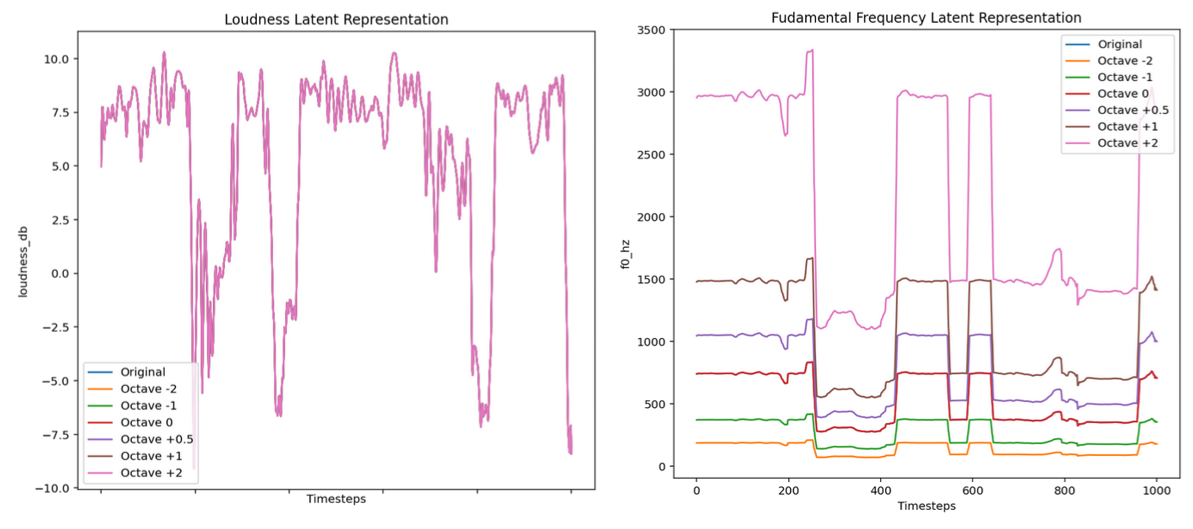
\includegraphics[width=\textwidth]{research/results/Coldplay/InferredTranspositionsGraphs.png}
    \caption{(Coldplay) Latent F0 and loudness features for various octave transpositions realative to F0 over timesteps throughout the frame}
\end{figure}

\subsection{Fixing F0}

The final pitch related test was fixing F0 to the mean value of F0 throughout the frame to see how the models would perform under unnatural pitch conditions.

Both models were able to fix pitch to the mean value of F0 in the frame. This is clearly heard and can be seen visibily from the inferred spectrogram images where the harmonic components are at lines of constant frequency, unlike the orginial where they clearly vary.

Additionally, words were still able to be synthesized and accurately heard, suggesting the model was able to learn the underlying phonemes of speech.

This is a very good result mimicking what was founded in the speech DDSP research\cite{SpeechDDSP} (whose code wasn't publicly available). Further experimentations were done to vary the pitch to other amounts eg 100Hz, 500Hz etc. to similar degrees of success, however the quality of results broke down at the extremes. This was evidenced by the harmonic again sounding more like a separate sound with the whispers producing the actual words.

Sadly, timbral quality was reduced when F0 was fixed, with the output sounding more robotic and the original timbre was lost. This is to be expected however as the original harmonic plus noise model was not designed with timbre transfer specifically in mind\cite{OriginalDDSP}.

\begin{figure}[H]
    \centering
    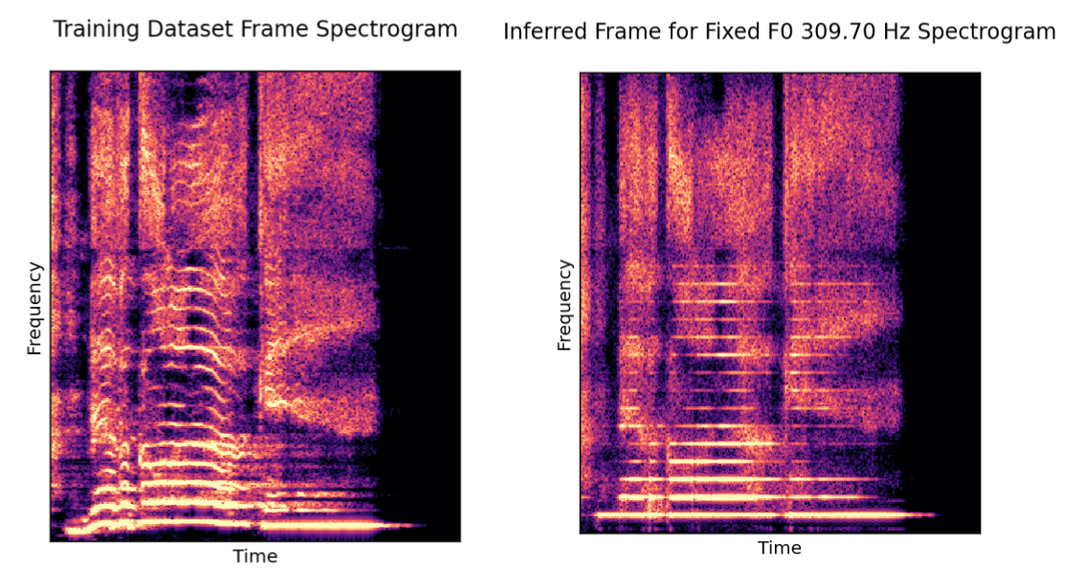
\includegraphics[width=\textwidth]{research/results/TaylorSwift/FixedF0.png}
    \caption{(Taylor Swift) Training dataset and fixed F0 spectrogram frames}
\end{figure}

\begin{figure}[H]
    \centering
    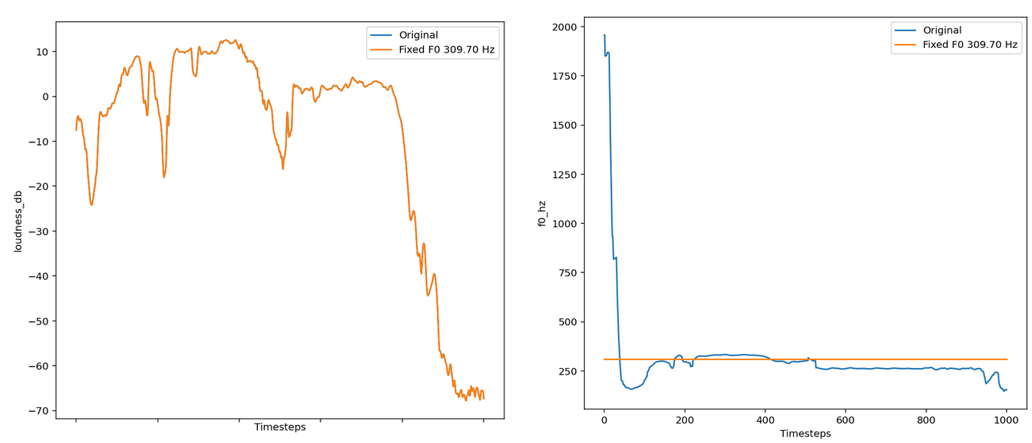
\includegraphics[width=\textwidth]{research/results/TaylorSwift/FixedF0Graphs.png}
    \caption{(Taylor Swift) Latent information on loudness and F0 over timesteps throughout the frame. The mean F0 was used to fix F0 throughout the frame}
\end{figure}

\begin{figure}[H]
    \centering
    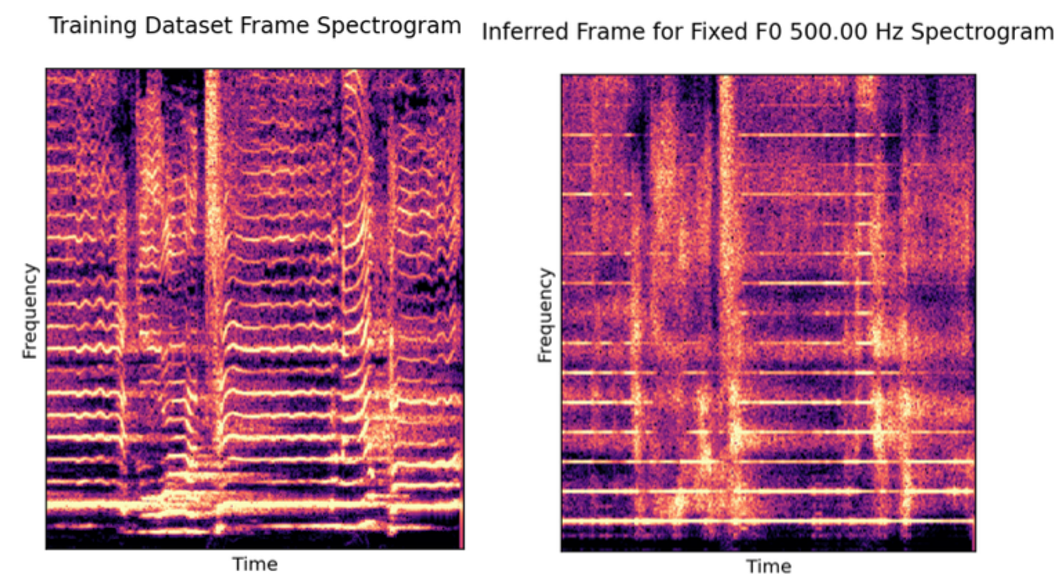
\includegraphics[width=\textwidth]{research/results/Coldplay/FixedF0.png}
    \caption{(Coldplay) Training dataset and fixed F0 spectrogram frames}
\end{figure}

\begin{figure}[H]
    \centering
    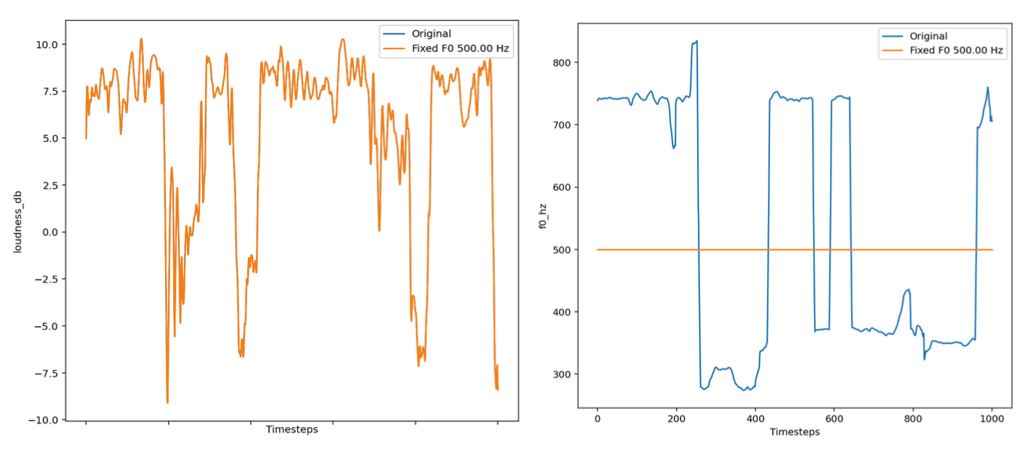
\includegraphics[width=\textwidth]{research/results/Coldplay/FixedF0Graphs.png}
    \caption{(Coldplay) Latent information on loudness and F0 over timesteps throughout the frame. The mean F0 was used to fix F0 throughout the frame}
\end{figure}

\subsection{Modifying Loudness}

Unfortunately modification of the loudness latent vector did not alter the loudness of any inferred frames. This could be caused by the decoder learning to ignore the loudness latent vector as it seemed insignificant.

Alternatively there may be some archtectural issue with modified decoder as the DDSP library's authors significantly redesigned the loudness and power and calculations with the version 3 release, this is since the release of the Singing DDSP decoder that used DDSP version 1. The discovery of which is beyond the scope of this paper.

\subsection{Timbral Transfer}

Following the success of the pitch related tests, several tests were conducted. The Taylor Swift model was selected for this due to its greater perceived performance in the pitch transfer tests.

\begin{enumerate}
    \item An unseen female voice timbral transfer was conducted using the song Deep End\cite{Birdy}. 
    \item Unseen male voice timbral transfer. 
\end{enumerate}

\subsection{General Problems}

Along with the loudness perception problem, there were others that were ecounterred during all inferencing tests:

\begin{enumerate}
    \item At low loudness levels, the CREPE model was not able to accurately detect pitch of the audio sample, this caused the fudamental ferquency to jump around, sometimes appearing to jump up an octave. This made the output sound jarring. This is evidenced in the Coldplay Frames that all experience this problem. A potential solution that the DDSP authors suggested was muting sections of track where CREPE had low confidence in it's prediction. This was unable to work here due to the problems discussed around the loudness latent.
    \item The model failed to learn specific timbre related to the trained artist, this was respecially appearent during the fixed F0 test when the output sounded almost robotic. This is in part expected as the DDSP archtecture was not designed with timbre transfer directly in mind.
    \item Similarly, when transferring timbre from another artist, the inferred sample sounded like the voice of the other artist more than it did that of the training dataset artist. This could however just be attributed to the generalisation of the model to resynthesizing the specific timbres derived from the noise characteristics of a test frame.
\end{enumerate}